% TEMPLATE for Usenix papers, specifically to meet requirements of
%  USENIX '05
% originally a template for producing IEEE-format articles using LaTeX.
%   written by Matthew Ward, CS Department, Worcester Polytechnic Institute.
% adapted by David Beazley for his excellent SWIG paper in Proceedings,
%   Tcl 96
% turned into a smartass generic template by De Clarke, with thanks to
%   both the above pioneers
% use at your own risk.  Complaints to /dev/null.
% make it two column with no page numbering, default is 10 point

% Munged by Fred Douglis <douglis@research.att.com> 10/97 to separate
% the .sty file from the LaTeX source template, so that people can
% more easily include the .sty file into an existing document.  Also
% changed to more closely follow the style guidelines as represented
% by the Word sample file. 

% Note that since 2010, USENIX does not require endnotes. If you want
% foot of page notes, don't include the endnotes package in the 
% usepackage command, below.

% This version uses the latex2e styles, not the very ancient 2.09 stuff.
\documentclass[letterpaper,twocolumn,10pt]{article}
\usepackage{usenix,epsfig,endnotes}
\usepackage[T1]{fontenc}
\begin{document}

%don't want date printed
\date{}

%make title bold and 14 pt font (Latex default is non-bold, 16 pt)
\title{\Large \bf Building a Modular ROS Network for the Raven II}

%for single author (just remove % characters)
\author{
{\rm Troy\ Sankey}\\
University of California Los Angeles
\and
{\rm Qu\ (Jackie)\ Jin}\\
University of California Los Angeles
\and
{\rm Jonathan\ Chan}\\
University of California Los Angeles
} % end author

% \maketitle

\twocolumn[
  \begin{@twocolumnfalse}
    \maketitle
    \begin{abstract}

This is the abstract. This is the abstract. This is the abstract.
This is the abstract. This is the abstract. This is the abstract.
This is the abstract. This is the abstract. This is the abstract.
This is the abstract. This is the abstract. This is the abstract.
This is the abstract. This is the abstract. This is the abstract.
\\

    \end{abstract}
  \end{@twocolumnfalse}
]


% Use the following at camera-ready time to suppress page numbers.
% Comment it out when you first submit the paper for review.
% \thispagestyle{empty}


\section{Introduction}
The Raven II surgical robotic arm was designed by the BioRobotics
Laboratory (BRL) at the University of Washington, and one copy of the
robot was given to the Center for Advanced Surgical and Interventional
Technology (CASIT) at the University of California Los Angeles to help
study and improve. I worked in a team of three people---together with
Jonathan Chan and Jackie Jin---to help modularize the code base of the
Raven II as provided by BRL.

In computer science, using modular design guarantees code readability
and, most importantly, code shareability. The Raven II implements
Robot Operating System (ROS) which is a programming framework built
around the idea of modular components that are, in theory, so abstract
that they can even be shared across different robots. However, we
discovered that BRL's use of ROS programming constructs are minimal
(granted, ROS did not exist when the Raven was originally conceived).

\section{Motivation}

\subsection{Robots in MIS, and software}

\subsection{Understanding the Raven code}
The structure of the current raven system is straightfoward. At the
highest level, there is a master node and a slave node. The master
interprets the position and orientation of two Phantom Omni haptic
controllers (for both arms), translates them into a differential
position and orientation, then transmits that to the slave. The slave
will accumulate the differential pose\footnote{in robotics, \emph{pose}
  is the combination of position and orientation} into an absolute
pose, or goal pose, then attempt to reach the goal pose.

For the slave, this process repeats every millisecond. The master is
on its own time---there is no synchronization between the master and
slave.

The slave code spawns three threads:

\begin{itemize}
  \item console I/O
  \item networking
  \item control (e.g. IK, ATMEL I/O)
\end{itemize}

Control is a realtime thread that, at a fixed interval, reads from and
writes to the ATMEL on the two raven PCB's.

\subsection{Lack of modular design in the Raven code}

\subsection{Image recognition}

\subsection{No-fly zones}

\subsection{Arbitrary controllers}

\section{Requirements}

\section{Design}

\begin{figure*}[t]
\begin{center}
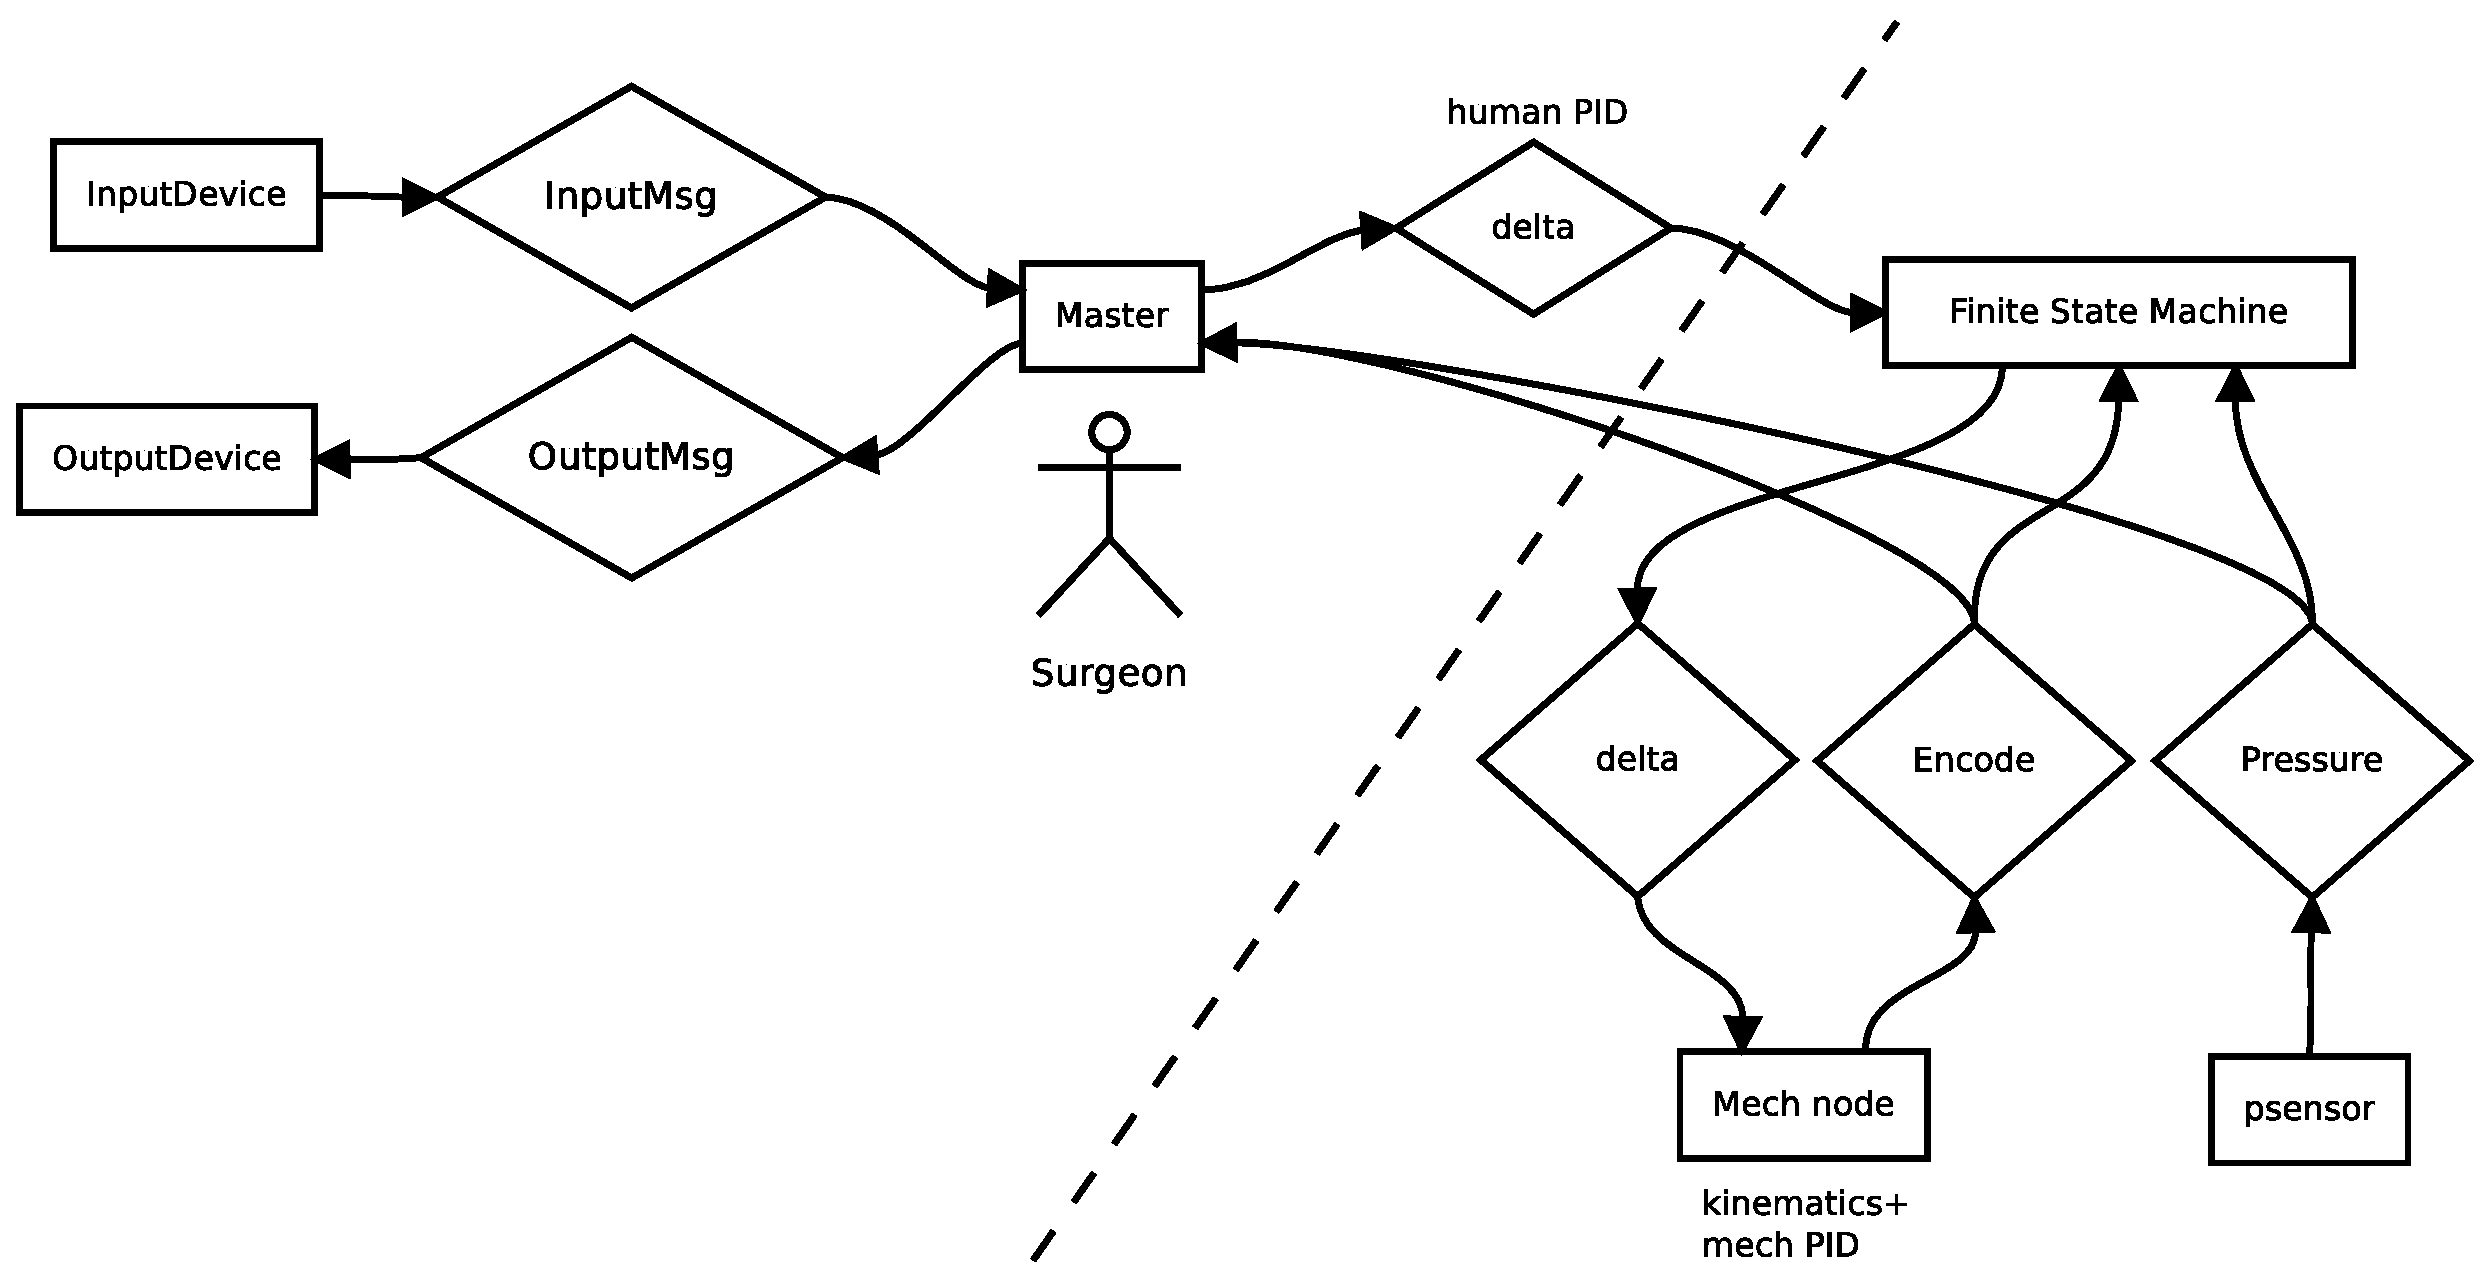
\includegraphics[width=1.0\textwidth]{ros_high_level_v2.eps}
\end{center}
\caption{Wonderful Flowchart}
\end{figure*}

\section{Mistakes}

\section{Conclusion}


%% {\footnotesize \bibliographystyle{acm}
%% \bibliography{../common/bibliography}}

%% \theendnotes

\end{document}
